
\chapter{Data Calibrated using Weights Derived from Monte Carlo}
\label{MC_weights_appendix}
The results presented in Chapter~\ref{chapTB} use weights derived from data to calibrate the simulation results.
In figure~\ref{dataMCweightfig} the response to hadrons, obtained from data, is plotted as a function of beam energy, for cylindrical and topological clusters at positions 4L and 4H. These plots include results obtained when the weights used for hadronic calibration are derived from the simulation, rather than data. This is analogous to the hadronic calibration schemes used at \atlas, in that the data is calibrated using results obtained from simulations. 

\begin{figure}[hb]
\begin{center}
\subfigure{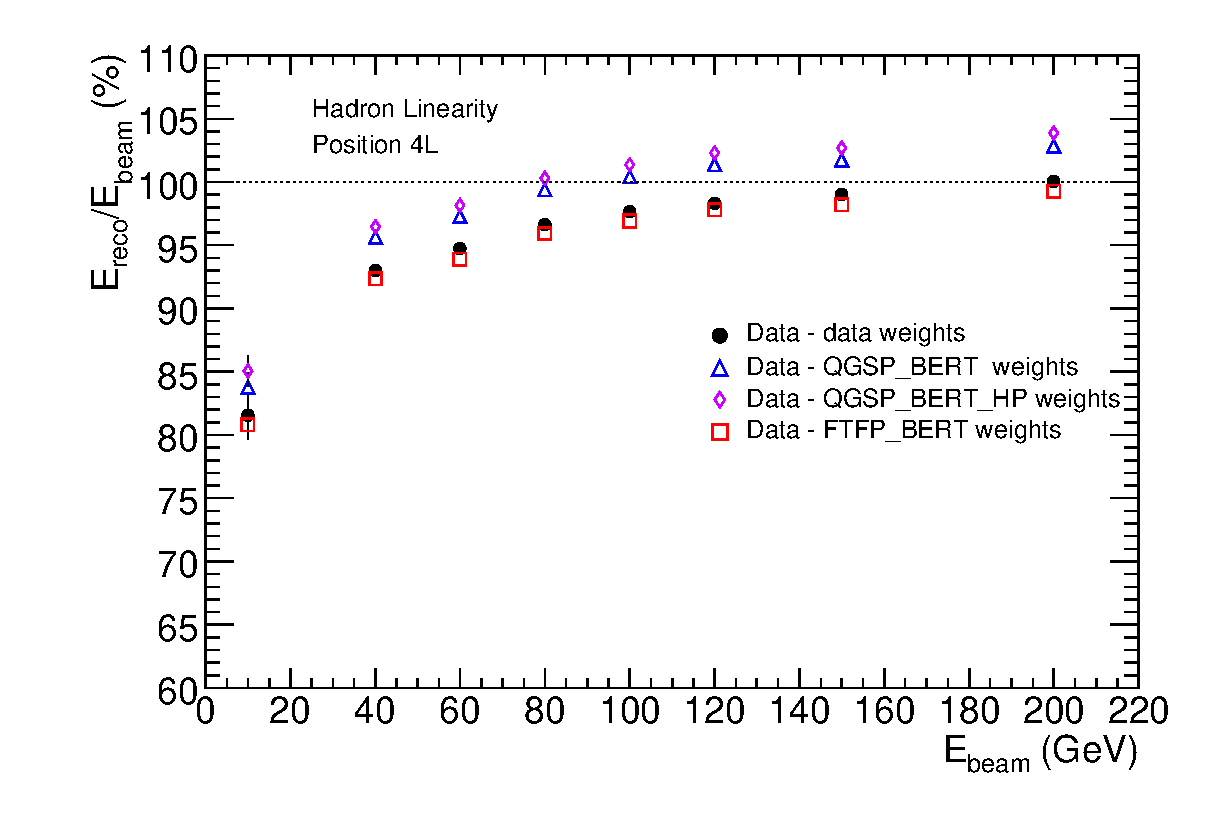
\includegraphics[width=0.45\linewidth,angle=0]{FCalTB_plots/hadron_linearity_4L_dataMCweights.eps}}
\subfigure{\includegraphics[width=0.45\linewidth,angle=0]{FCalTB_plots/hadron_linearity_4H_dataMCweights.eps}}\\
\subfigure{\includegraphics[width=0.45\linewidth,angle=0]{FCalTB_plots/hadron_linearity_4L_t420_dataMCweights.eps}}
\subfigure{\includegraphics[width=0.45\linewidth,angle=0]{FCalTB_plots/hadron_linearity_4H_t420_dataMCweights.eps}}\\
\end{center}
\caption[Hadron data calibrated with MC-derived weights.]{The FCal response to hadrons at positions 4L (a,c) and 4H (b,d), using cylindrical (a,b) and topological (c,d) clusters. The solid black markers show the results obtained from data, in which the flat weights used for hadronic calibration are also derived from data. The open markers show the results obtained when weights derived from Monte Carlo are used to calibrate the data.}
\label{dataMCweightfig}
\end{figure}

